\documentclass[a4paper,11pt,BCOR10mm,oneside,headsepline]{scrartcl}
\usepackage{amsmath, mathtools}
\usepackage[ngerman]{babel}
\usepackage[utf8]{inputenc}

\usepackage{typearea, url}
\areaset{17cm}{26cm}
\setlength{\topmargin}{-1cm}
\usepackage{scrpage2}
\pagestyle{scrheadings}

\usepackage[T1]{fontenc}
\usepackage{beramono}
\usepackage{listings}
\usepackage[usenames,dvipsnames]{xcolor}
\usepackage{graphicx}
\usepackage{subcaption}

\ihead{HW6: CIS 631, Parallel Processing}
\ohead{\pagemark}
\chead{}
\cfoot{}

\begin{document}
	
	\begin{center}
		\textbf{\large Homework 6 Report}
	\end{center}\vskip1em
	
	\section{Test Environment}
	I tested my code on a Google Compute Instance with NVIDIA Tesla V100 GPU, with CUDA 11.1.
		
	\section{Experiments and Results}
		\subsection{CG using CSR}
		Max iteration: 20,000 Tolerance: 1e-6\\
		Number of blocks: (m + threads - 1) / threads\\

		\begin{table}[!htbp]
			\centering
			\begin{tabular}{|c|c|c|}
				\hline
				\textbf{Threads Per Block} & \textbf{Time (seconds)} & \textbf{norm of (b - A * x)} \\ \hline
				32                         & 8.132622                & 4.43E-05                     \\ \hline
				64                         & 7.928369                & 4.43E-05                     \\ \hline
				128                        & 7.867733                & 4.43E-05                     \\ \hline
				256                        & 8.048368                & 4.43E-05                     \\ \hline
				512                        & 6.907522                & 4.43E-05                     \\ \hline
				1024                       & 10.923411               & 4.43E-05                     \\ \hline
			\end{tabular}
			\caption*{Table 1.CG using CSR}
		\end{table}
		
		\subsection{CG using ELL (row-major with shared memory)}
		The skeleton code converts CSR to ELL by storing the first row, the second row, ..., the last row into the 1-D array.\\
		Max iteration: 20,000 Tolerance: 1e-6\\
		Number of blocks: m\\
		
		\begin{table}[!htbp]
			\centering
			\begin{tabular}{|c|c|c|}
				\hline
				\textbf{Threads Per Block} & \textbf{Time (seconds)} & \textbf{norm of (b - A * x)} \\ \hline
				32                         & 4.029764                & 6.45E-05                     \\ \hline
				64                         & 3.77639                 & 5.27E-05                     \\ \hline
				128                        & 4.523906                & 4.93E-05                     \\ \hline
				256                        & 6.740506                & 4.93E-05                     \\ \hline
				512                        & 12.004819               & 4.93E-05                     \\ \hline
				1024                       & 25.205187               & 4.93E-05                     \\ \hline
			\end{tabular}
			\caption*{Table 2.CG using ELL (row-major with shared memory)}
		\end{table}
		
		\newpage
		\subsection{CG using ELL (column-major without shared memory)}
		Most ELL format uses column-major format. This is also the way I converted CSR to ELL for homework5. It stores the first column, second column, ..., the last column into the 1-D array.\\
		Max iteration: 20,000 Tolerance: 1e-6\\
		Number of blocks: m\\
		
		\begin{table}[!htbp]
			\centering
			\begin{tabular}{|c|c|c|}
				\hline
				\textbf{Threads Per Block} & \textbf{Time (seconds)} & \textbf{norm of (b - A * x)} \\ \hline
				32                         & 3.718985                & 4.43E-05                     \\ \hline
				64                         & 3.690877                & 4.43E-05                     \\ \hline
				128                        & 3.677182                & 4.43E-05                     \\ \hline
				256                        & 3.682065                & 4.43E-05                     \\ \hline
				512                        & 3.685367                & 4.43E-05                     \\ \hline
				1024                       & 4.24437                 & 4.43E-05                     \\ \hline
			\end{tabular}
			\caption*{Table 3.CG using ELL (column-major without shared memory)}
		\end{table}
		
		\subsection{CG using ELL (column-major with shared memory)}
		This one tests column-major ELL with shared memory.\\
		Max iteration: 20,000 Tolerance: 1e-6\\
		Number of blocks: m\\
		
		\begin{table}[!htbp]
			\centering
			\begin{tabular}{|c|c|c|}
				\hline
				\textbf{Threads Per Block} & \textbf{Time (seconds)} & \textbf{norm of (b - A * x)} \\ \hline
				32                         & 9.118011                & 6.45E-05                     \\ \hline
				64                         & 9.165521                & 5.27E-05                     \\ \hline
				128                        & 9.534499                & 4.93E-05                     \\ \hline
				256                        & 10.45859                & 4.93E-05                     \\ \hline
				512                        & 13.044246               & 4.93E-05                     \\ \hline
				1024                       & 24.3799                 & 4.93E-05                     \\ \hline
			\end{tabular}
			\caption*{Table 4.CG using ELL (column-major with shared memory)}
		\end{table}
		
		\subsection{Larger Max Iterations}
		This tests the error for CSR and ELL vs. different max iteration.
		\begin{table}[!htbp]
			\centering
			\begin{tabular}{|c|c|c|}
				\hline
				\textbf{Max Iteration} & \textbf{CSR Error} & \textbf{ELL Error} \\ \hline
				13000                  & 9.891570e-04       & 9.891570e-04       \\ \hline
				14000                  & 2.109754e-03       & 2.109754e-03       \\ \hline
				16000                  & 4.004684e-04       & 4.004684e-04       \\ \hline
				18000                  & 1.920288e-04       & 1.920288e-04       \\ \hline
				20000                  & 4.431995e-05       & 4.431995e-05       \\ \hline
				22000                  & 1.261112e-04       & 1.261112e-04       \\ \hline
			\end{tabular}
			\caption*{Table 5. Error vs. Max Iteration}
		\end{table}
		
		\newpage
		\subsection{Performance Comparison}
		\begin{figure}[!htbp]
			\centering
			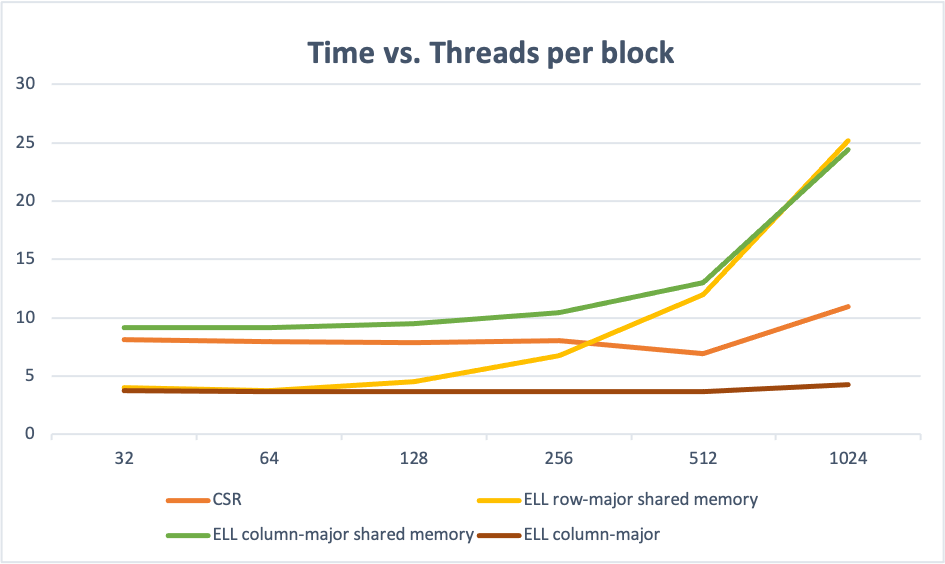
\includegraphics[scale=0.6]{plot}
			\caption*{Figure 1. Performance Comparison}
		\end{figure}
		
	\section{Findings}
		\begin{itemize}
			\item ELL (column-major without shared memory) takes ~1/2 time than CSR. This is because ELL uses padding to store the non-zero elements to store non-zero elements contiguously. By allowing coalesced memory access, it outperforms CSR. The trade-off is that ELL will end up taking more space to store the sparse matrix than CSR.
			\item By using row-major format ELL with shared memory, it performs slightly worse than column-major format ELL without shared memory. However, it performs better than column-major format with shared memory.
			\item When max iteration is 20,000, CG has the lowest error for CSR and ELL. 
		\end{itemize}
	
\end{document}